%! Author = tstreule

\section{Recurrent Neural Networks}\label{sec:recurrent-nns}


\begin{formula}{Linear RNN}
    $\highlight{\symbf h^t} = F(\symbf h^{t-1}, \symbf x^t; \symbf\theta)$,\enskip $\highlight{\symbf h^0} = \symbf 0$,\enskip $F = \sigma \circ \bar F$ \\
    $\bar F(\symbf{h, x; \theta}) = \symbf{Wh + Ux + b}$,\enskip $\symbf\theta = (\symbf{U, W, b, \ldots})$ \\
    \llap{\textit{optional:\enskip}}$\symbf y = H(\symbf{h; \theta})$,\enskip $H(\symbf{h; \theta}) \coloneqq \sigma(\symbf{Vh + c})$,\enskip $\symbf\theta = (\ldots, \symbf{V, c})$
\end{formula}

You can loot at is as a neural network. However, the first input has $N$ layers, the second $N\shortminus1$, etc., and the last has two layers.

\begin{figure}[H]
    \label{fig:unfold-rnn}
    \centering
    %! Author = tstreule

\begin{scriptsize}
\begin{tikzpicture}[
    >=stealth, % default arrow style
    every node/.append style={inner sep=0.5pt},
    every path/.append style={-stealth, thick, shorten >=0.5pt}
]
\tikzstyle{place}=[circle, draw=black, minimum size=2.5em]

% --- "rolled" RNN ---

    \node[place] (y) at (0,2) {$\symbf y$};
    \node[place] (h) at (0,1) {$\symbf h$};
    \node[place] (x) at (0,0) {$\symbf x$};
    \draw (x) --node[left=2pt] {$\symbf U$} (h);
    \draw (h) --node[left=2pt] {$\symbf V$} (y);

    \node[fill=black,minimum size=0.5em] (W) at (0.7,1) {};
    \node[right=0cm and 0cm of W] {$\symbf W$};
    \draw (h) to[out=-45,in=-90,looseness=1.5] (W) to[out=90,in=45,looseness=1.5] (h);

% --- Rightarrow "unroll"

    \draw (1.35,1) --node[above=2pt] {unroll~~~} (2.45,1);

% --- unrolled RNN ---

    % all y's
    \node[place] (yt-1) at (4,2) {$\symbf y^{t\shortminus1}$};
    \node[place] (yt)   at (5,2) {$\symbf y^{t}$};
    \node[place] (yt+1) at (6,2) {$\symbf y^{t+1}$};
    % all h's
    \node[place] (ht-2) at (3,1) {$\symbf h^{t\shortminus2}$};
    \node[place] (ht-1) at (4,1) {$\symbf h^{t\shortminus1}$};
    \node[place] (ht)   at (5,1) {$\symbf h^{t}$};
    \node[place] (ht+1) at (6,1) {$\symbf h^{t+1}$};
    \node[place] (ht+2) at (7,1) {$\symbf h^{t+2}$};
    % all x's
    \node[place] (xt-1) at (4,0) {$\symbf x^{t\shortminus1}$};
    \node[place] (xt)   at (5,0) {$\symbf x^{t}$};
    \node[place] (xt+1) at (6,0) {$\symbf x^{t+1}$};

    % h-h connections (horizontal)
    \draw (ht-2) --node[above=2pt] {$\gray\symbf W$} (ht-1);
    \draw (ht-1) --node[above=2pt] {$\gray\symbf W$} (ht);
    \draw (ht)   --node[above=2pt] {$\gray\symbf W$} (ht+1);
    \draw (ht+1) --node[above=2pt] {$\gray\symbf W$} (ht+2);
    % x-h connections (vertical)
    \draw (xt-1) --node[left=2pt] {$\gray\symbf U$} (ht-1);
    \draw (xt)   --node[left=2pt] {$\gray\symbf U$} (ht);
    \draw (xt+1) --node[left=2pt] {$\gray\symbf U$} (ht+1);
    % h-y connections (vertical)
    \draw (ht-1) --node[left=2pt] {$\gray\symbf V$} (yt-1);
    \draw (ht)   --node[left=2pt] {$\gray\symbf V$} (yt);
    \draw (ht+1) --node[left=2pt] {$\gray\symbf V$} (yt+1);

\end{tikzpicture}
\end{scriptsize}

\end{figure}

\textbf{Backpropagation through time:}
\begin{itemize}
    \item Propagate derivates backwards through time
    \item Parameter sharing leads to a sum over $t$
    \item \textit{Def.} shortcut $\dot\sigma_i^t \coloneqq \sigma' (\bar F_i (h^{t\shortminus1}, x^t))$,\enskip $\symbf S(\symbf h^r) = \diag(\dot\sigma_1^r, {\ldots}, \dot\sigma_n^r)$
    \item \textbf{RNN gradients:} $\nabla_{\symbf x^t} \mathcal R = \brack*{\prod_{r=t+1}^s \symbf{W^\top S}(\symbf h^r)} \cdot \symbf J_H \cdot \nabla_{\symbf y} \mathcal R$
\end{itemize}


% ===
\subsection{Memory Units -- LSTM}

Classical RNNs easily forget (info gets ``washed out'').

\begin{figure}[H]
    \label{fig:lstm}
    \centering
    \begin{flushleft}
        \color{BlueViolet}\sffamily\scriptsize
        \quad (1): element-wise, to (not) pass information,\\
        \quad (2): add info to memory $C_t$
    \end{flushleft}\vspace{-2em}
    %! Author = tstreule

\begin{tikzpicture}[
    % Global config
    font=\sffamily,
    >=stealth, % default arrow style
    x=8mm,
    y=7mm,
    % Styles
    cell/.style={% the main box
        rectangle, rounded corners=4mm,
        draw=lime!70!teal!80, very thick,
        fill=lime!70!teal!20,
    },
    operator/.style={% operators like 'plus/+' or 'multiply/x'
        circle, inner sep=-.5pt,
        draw, fill=red!25,
    },
    function/.style={% functions like 'tanh'
        operator,% inherit style
        ellipse, inner sep=.5pt,
    },
    external/.style={% external in-/outputs
        inner sep=1pt,
    },
    knot/.style={% internal knots
        rectangle, inner sep=1.5pt,
        minimum width=5mm, minimum height=1em,
        draw, fill=yellow!35,
    },
    rigidArrow/.style={% arrows w/ tight corners
        rounded corners=.75mm,
        very thick,
    },
    roundArrow/.style={% arrows w/ big rounded corners
        rigidArrow,% inherit style
        rounded corners=2mm,
    },
    reference/.style={% text for reference
        rectangle, color=BlueViolet, fill=white, fill opacity=0.8,
        inner sep=1pt, outer sep=1pt,
    },
]

% Draw elements
    % Draw the cell / main box
    \node [cell, above right, minimum width=50mm, minimum height=24mm] at (0,0) {};

    % Draw internal knots --- knot-#
    \node [knot] (knot-1) at (1,1) {$\sigma$};
    \node [knot] (knot-2) at (2,1) {$\sigma$};
    \node [knot] (knot-3) at (3,1) {\scriptsize tanh};
    \node [knot] (knot-4) at (4,1) {$\sigma$};

    % Draw operators --- mul-# , sum-# , fct-#
    \newcommand{\myplus}{\scalebox{.9}{$+$}}
    \node [operator] (mul-1) at (1,3) {$\times$};
    \node [operator] (sum-1) at (3,3) {\myplus};
    \node [operator] (mul-2) at (3,2) {$\times$};
    \node [operator] (mul-3) at (5,2) {$\times$};
    \node [function] (fct-1) at (5,2.6) {\scriptsize tanh};
    \node [reference, above=0mm of mul-1] {\scriptsize(1)};
    \node [reference, above=0mm of sum-1] {\scriptsize(2)};

    % Draw inputs --- c-in , h-in, x
    \node [external] (c-in) at (-1,3) {};
    \node [external, above right=0pt and 0pt of c-in] {$C_{t\shortminus1}$};
    \node [external] (h-in) at (-1,.4) {};
    \node [external, above right=0pt and 0pt of h-in] {$h_{t\shortminus1}$};
    \node [external] (x) at (.5,-.7) {};
    \node [external, above left=0pt and 0pt of x] {$x_t$};

    % Draw outputs --- c-out , h-out , h-out2
    \node [external] (c-out) at (7,3) {};
    \node [external, above=0pt of c-out] {$C_t$};
    \node [external] (h-out) at (7,.4) {};
    \node [external, above=0pt of h-out] {$h_t$};
    \node [external] (h-out2) at (6,4.2) {};
    \node [external, below left=0pt and 1pt of h-out2] {$h_t$};

% Connect elements
    % dotted lines
    \draw [dotted, rigidArrow] (c-in) -- ++(-0.5,0);
    \draw [dotted, rigidArrow] (h-in) -- ++(-0.5,0);
    \draw [dotted, rigidArrow] (c-out) -- ++(0.5,0);
    \draw [dotted, rigidArrow] (h-out) -- ++(0.5,0);

    % inward connections
    \draw [->, rigidArrow] (c-in) -- (mul-1) -- (sum-1) -- (c-out);
    \draw [->, rigidArrow] (h-in) -| (knot-1) --node[left]{\scriptsize$f_t$} (mul-1);
    \draw [- , rigidArrow] (h-in) -| (knot-2);
    \draw [->, rigidArrow] (h-in) -| (knot-3) --node[right]{\scriptsize$\tilde C_t$} (mul-2);
    \draw [->, rigidArrow] (mul-2) -- (sum-1);
    \draw [->, roundArrow] (h-in) -| (knot-4) |-node[above=-1mm]{\scriptsize $o_t$} (mul-3);
    \draw [->, roundArrow] (knot-2) |-node[above=-1mm]{\scriptsize$i_t$} (mul-2);
    \draw [- , rigidArrow] (x) -- (x |- h-in) -| (knot-1);

    % outward connections
    \draw [- , rigidArrow] (sum-1) -| (fct-1) -- (mul-3);
    \draw [->, roundArrow] (mul-3) |- (h-out);
    \draw (c-out -| h-out2) ++(0,-0.15) coordinate (i1); % find intersection
    \draw [- , roundArrow] (h-out -| h-out2)++(-.5,0) -| (i1);
    \draw [->, roundArrow] (i1)++(0,0.3) -- (h-out2);

\end{tikzpicture}
%    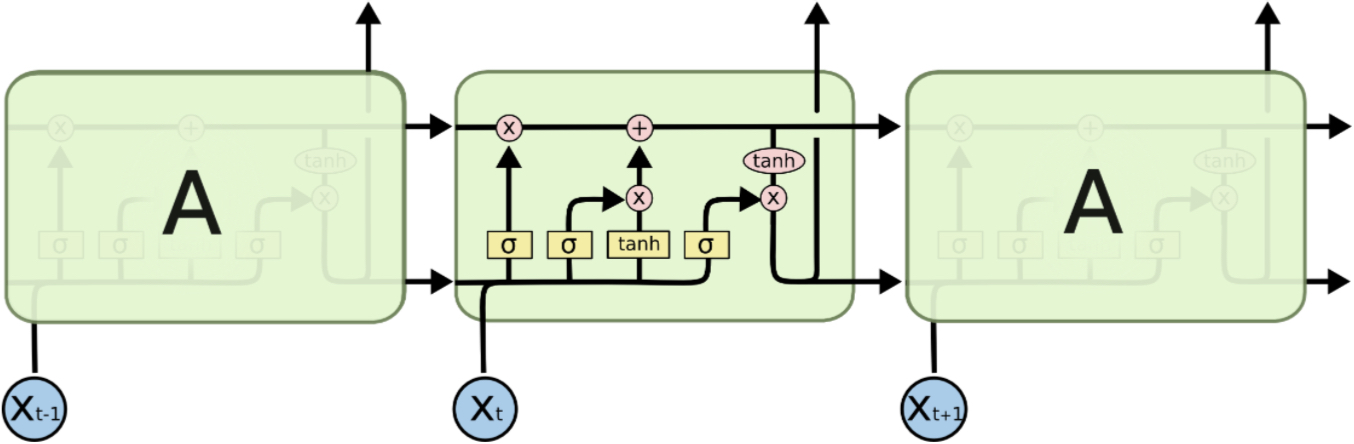
\includegraphics[width=.8\linewidth]{lstm_architecture}
\end{figure}

\begin{itemize}
    \item Information propagates along the chain
    \item can flow unchanged, only selectively changed by $\sigma$-gates
    \item can forget (when $f_t \approx 0$)
    \item LSTMs and GRUs can learn active memory strategies
    \item difficult to understand and resource-hungry
\end{itemize}


% ===
\subsection{Seq2Seq learning}

\textbf{Encoder RNN} $\symbf x \mapsto \symbf z$ and
\textbf{Decoder RNN} $\symbf z \mapsto \symbf y^{1:S}$ e.g. use encoder output as input for decoder and stop symbol \texttt{<EOS>}.

Can use Seq2Seq also for \textbf{image-to-text} sequencing, \ldots!


\textbf{Downsides of RNN:} (i) they don't work well for longer sequences, (ii) cannot be parallelized since architecture is sequential.
